%=====
\section{Case Study}

The proof concept of the proposed trace analysis method is demonstrated on a transaction level model of a simple SoC design with two CPU cores, memory, and a peripheral device connected by an interconnect as shown in Fig.~\ref{fig-SoC-ex}.  Since the analysis method presented in this paper is communication centric, the detailed computations of these blocks are not modeled.  Instead, the modeling is focused on how they participate in flows for different system level use cases.

\begin{figure}[tb]
\begin{center}
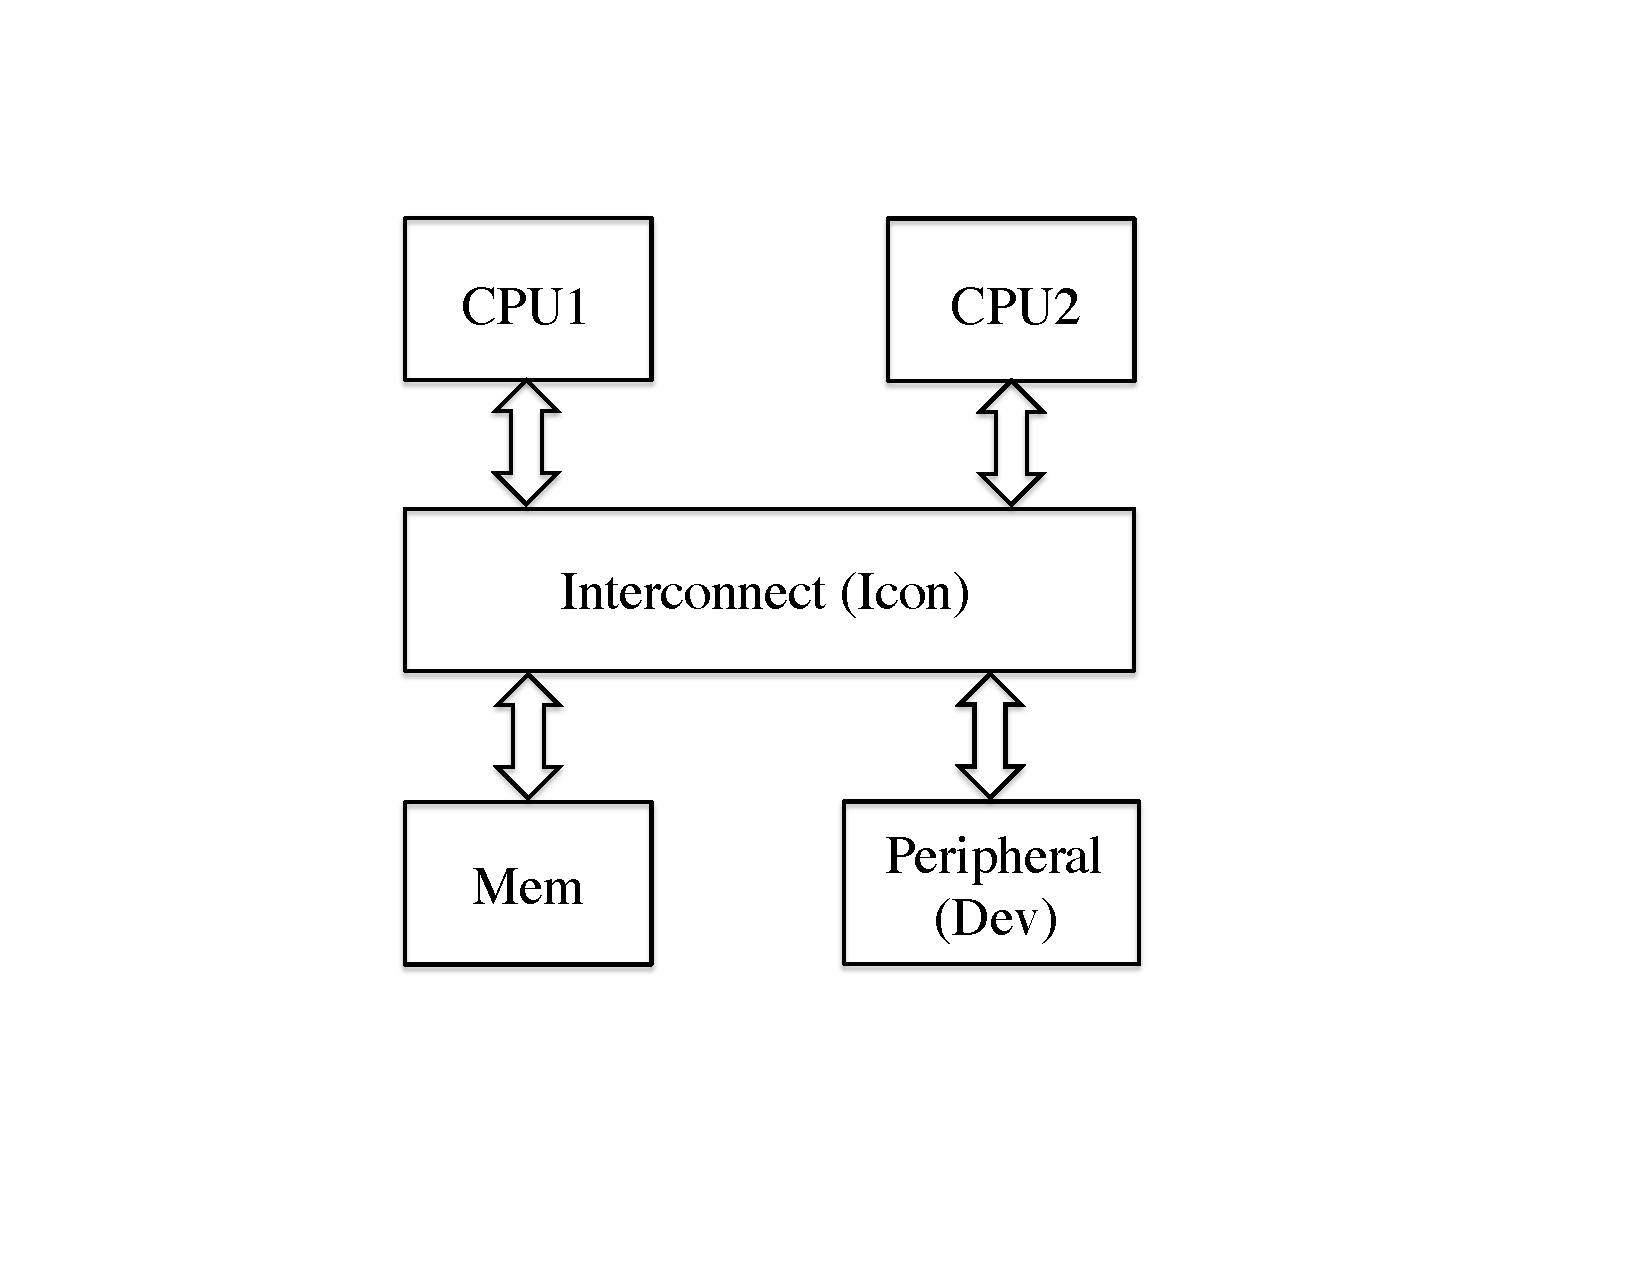
\includegraphics[width=2in]{figures/simple-ex}
\caption{A simple SoC example.}
\label{fig-SoC-ex}
\end{center}
\end{figure}


\subsection{Flow Specification}

In this case study, four system flows are implemented in the simple SoC model. They include cache coherent memory access operations and a memory-mapped peripheral read operation initiated from the CPUs, a message signaled interrupt operation initiated from the peripheral device.  These flow specifications capture how messages are exchanged for different use cases.  In this model, a message is defined with the following format, $(\mbox{Src}, \mbox{Dest}, \mathit{Cmd}, \mathit{Addr})$, where Src and Dest refer to the source and destination components of messages, $\mathit{Cmd}$ refers to the operations that the destination component should perform, and $\mathit{Addr}$ refers to memory addresses where $\mathit{Cmd}$ applies.  $\mathit{Cmd}$ can be memory accesses or not.  If it is not, then the $\mathit{Addr}$ field of messages is ignored.  In this case study, memory mapped IO mechanism is used.  Furthermore, detailed memory addresses are not modeled. Instead, the address space is partitioned to main memory addresses and peripheral addresses.  In messages, the $\mathit{Addr}$ field is replaced with either $M$ representing a memory address or $P$ representing an address to a peripheral device.  

The LPN as shown in Fig.~\ref{fig-cpu-write} specifies a system flow where {CPU2} initiates a memory write operation.   In this flow, CPU2 initiates a memory write request followed by a data valid message to the interconnect.  The data valid messages are used to model availability or validity of data for transfer.  Concurrently, the interconnect inquiries CPU1 if it holds a more updated version of the data by sending a memory write message $\mathit{msg_2}$.   CPU1 generates one of two possible responses.  If CPU1 holds the more updated data in its cache in the same memory space that CPU2 intends to write, a cache hit message $\mathit{msg_4}$ followed by $\mathit{msg_6}$ are sent to the interconnect.  Otherwise, CPU1 sends a cache miss message $\mathit{msg_5}$.  After getting the response from CPU1, Interconnect sends a write request to the memory unit.  This flow is symmetric for CPU1.

\begin{figure}[tb]
\begin{center}
\resizebox{2.8in}{!}{
\begin{tikzpicture}[node distance=3cm, auto,>=latex', thick]
\tikzset{rectbox/.style={rectangle, draw, align=flush center,thick, minimum size = 6mm}}
\tikzset{circ/.style={circle, draw,thick}}
\tikzset{terminal/.style={circle, draw,line width=.8mm}}
\tikzset{weight3/.style={line width=.3mm}}
	% Nodes:
	\node[circ]		(p1) 		at (0,0) {$p_1$};
	\node[rectbox]	(msg1)	at	($(p1) + (0,-1.1)$) {$msg_1$};
	\node[circ] 	(p2) 		at ($(msg1) + (-3,0)$) {$p_2$};
	\node[circ] 	(p3) 		at ($(msg1) + (3,0)$) {$p_3$};
	\node[rectbox]	(msg2)	at	($(p2) + (0,-1.1)$) {$msg_2$};
	\node[rectbox]	(msg3)	at	($(p3) + (0,-1.5)$) {$msg_3$};
	\node[circ] 	(p4) 		at ($(msg2) + (0,-1.1)$) {$p_4$};
	\node[rectbox]	(msg4)	at	($(p4) + (0,-1.1)$) {$msg_4$};
	\node[rectbox]	(msg5)	at	($(p4) + (3,0)$) {$msg_5$};
	\node[circ] 	(p6) 		at ($(msg4) + (0,-1.1)$) {$p_6$};
	\node[circ] 	(p5) 		at ($(msg3) + (0,-1.4)$) {$p_5$};
	\node[rectbox,rotate=90]	(msg6)	at	($(p6) + (1.5,0)$) {$msg_6$};
	\node[circ] 	(p7) 		at ($(msg6) + (1.5,0)$) {$p_7$};
	\node[rectbox]	(msg7)	at	($(p5) + (0,-1.5)$) {$msg_7$};
	\node[terminal]	(p8)	at	($(msg7) + (2,0)$) {$p_8$};
	% Edges
	\draw[->,weight3]	(p1) -- (msg1);
	\draw[->,weight3]	(msg1) -- (p2);
	\draw[->,weight3]	(msg1) -- (p3);
	\draw[->,weight3]	(p2) -- (msg2);
	\draw[->,weight3]	(msg2) -- (p4);
	\draw[->,weight3]	(p4) -- (msg4);
	\draw[->,weight3]	(p4) -- (msg5);
	\draw[->,weight3]	(msg4) -- (p6);
	\draw[->,weight3]	(p6) -- (msg6);
	\draw[->,weight3]	(msg6) -- (p7);
	\draw[->,weight3]	(p7) -- (msg7);
	\draw[->,weight3]	(msg7) -- (p8);
	\draw[->,weight3]	(msg5) -- (p7);
	\draw[->,weight3]	(p3) -- (msg3);
	\draw[->,weight3]	(msg3) -- (p5);
	\draw[->,weight3]	(p5) -- (msg7);
	
	\node[]	(msg-def)	at	($(p1) + (0,-8.5)$) {
	\begin{minipage}{3in}
	Definition of the messages:
\[
\begin{array}{clllll}
msg_1: & (\mbox{CPU2},	& \mbox{Icon},		& \mathit{Wr}, 	& M) \\
msg_2: & (\mbox{Icon},	& \mbox{CPU1}, 	& \mathit{Wr},			& M) \\
msg_3: & (\mbox{CPU2},	& \mbox{Icon}, 	& \mathit{DVal},	& -) \\
msg_4: & (\mbox{CPU1},	& \mbox{Icon}, 	& \mathit{Hit},	& -) \\
msg_5: & (\mbox{CPU1},	& \mbox{Icon}, 	& \mathit{Miss},	& -) \\
msg_6: & (\mbox{CPU1},	& \mbox{Icon}, 	& \mathit{DVal},	& -) \\
msg_7: & (\mbox{Icon},	& \mbox{Mem}, 		& \mathit{Wr},			& M) \\
\end{array}
\]
\end{minipage}
		};
\end{tikzpicture}
}
\caption{Flow specification ($F_1$) of a cache coherent write operation initiated from \texttt{CPU2}.}
\label{fig-cpu-write}
\end{center}
\end{figure}


The LPN specification as shown in Fig.~\ref{fig-cpu-read} captures the system flow where CPU2 initiates a memory read operation.  Basically, CPU2 sends a memory read message to Interconnect, which then generates two concurrent threads, one checks if CPU1 has the more updated data in the memory space for the read operation, and the other thread to get data from the memory.  Once Interconnect gets both responses from CPU1 and memory, it synchronizes the responses, and writes the correct data to the CPU2's cache and memory in parallel.  Again, this specification is symmetric for CPU1.


\begin{figure}[htbp]
\begin{center}
\resizebox{3.2in}{!}{
\begin{tikzpicture}[node distance=3cm, auto,>=latex', thick]
\tikzset{rectbox/.style={rectangle, draw, align=flush center,thick, minimum size = 6mm}}
\tikzset{circ/.style={circle, draw,thick}}
\tikzset{terminal/.style={circle, draw,line width=.8mm}}
\tikzset{weight3/.style={line width=.3mm}}
	% Nodes:
	\node[circ]		(p1) 		at (0,0) {$p_1$};
	\node[rectbox]	(msg1)	at	($(p1) + (0,-1.1)$) {$msg_1$};
	\node[circ] 	(p2) 		at ($(msg1) + (-3,0)$) {$p_2$};
	\node[circ] 	(p3) 		at ($(msg1) + (2,0)$) {$p_3$};
	\node[rectbox]	(msg2)	at	($(p2) + (0,-1.1)$) {$msg_2$};
	\node[rectbox]	(msg3)	at	($(p3) + (2,0)$) {$msg_3$};
	\node[circ] 	(p4) 		at ($(msg2) + (0,-1.1)$) {$p_4$};
	\node[rectbox]	(msg4)	at	($(p4) + (0,-1.1)$) {$msg_4$};
	\node[rectbox]	(msg5)	at	($(p4) + (3,0)$) {$msg_5$};
	\node[circ] 	(p6) 		at ($(msg4) + (0,-1.1)$) {$p_6$};
	\node[circ] 	(p5) 		at ($(msg3) + (0,-1.1)$) {$p_5$};
	\node[rectbox,rotate=90]	(msg6)	at	($(p6) + (1.5,0)$) {$msg_6$};
	\node[circ] 	(p7) 		at ($(msg6) + (1.5,0)$) {$p_7$};
	\node[rectbox]	(msg7)	at	($(p5) + (0,-1.1)$) {$msg_7$};
	\node[circ]	(p8)	at	($(msg7) + (0,-1.1)$) {$p_8$};
	\node[rectbox]	(msg8)	at	($(p8) + (0,-1.1)$) {$msg_8$};
	\node[circ]	(p9)	at	($(msg8) + (-1.5,-1.1)$) {$p_9$};
	\node[circ]	(p10)	at	($(msg8) + (1.5,-1.1)$) {$p_{10}$};
	\node[rectbox]	(msg9)	at	($(p9) + (0,-1.1)$) {$msg_9$};
	\node[rectbox]	(msg10)	at	($(p10) + (0,-1.1)$) {$msg_{10}$};
	\node[terminal]	(p11)	at	($(msg9) + (0,-1.1)$) {$p_{11}$};
	\node[terminal]	(p12)	at	($(msg10) + (0,-1.1)$) {$p_{12}$};

	% Edges
	\draw[->,weight3]	(p1) -- (msg1);
	\draw[->,weight3]	(msg1) -- (p2);
	\draw[->,weight3]	(msg1) -- (p3);
	\draw[->,weight3]	(p2) -- (msg2);
	\draw[->,weight3]	(msg2) -- (p4);
	\draw[->,weight3]	(p4) -- (msg4);
	\draw[->,weight3]	(p4) -- (msg5);
	\draw[->,weight3]	(msg4) -- (p6);
	\draw[->,weight3]	(p6) -- (msg6);
	\draw[->,weight3]	(msg6) -- (p7);
	\draw[->,weight3]	(p7) -- (msg8);
	\draw[->,weight3]	(msg7) -- (p8);
	\draw[->,weight3]	(msg5) -- (p7);
	\draw[->,weight3]	(p3) -- (msg3);
	\draw[->,weight3]	(msg3) -- (p5);
	\draw[->,weight3]	(p5) -- (msg7);
	\draw[->,weight3]	(p8) -- (msg8);
	\draw[->,weight3]	(msg8) -- (p9);
	\draw[->,weight3]	(msg8) -- (p10);
	\draw[->,weight3]	(p9)  -- (msg9);
	\draw[->,weight3]	(p10)  -- (msg10);
	\draw[->,weight3]	(msg9) -- (p11);
	\draw[->,weight3]	(msg10) -- (p12);
	
	\node[]	(msg-def)	at	($(p1) + (-2.7,-10)$) {
	\begin{minipage}{2in}
	Definition of the messages:
\[
\begin{array}{clllll}
msg_1: & (\mbox{CPU2},	& \mbox{Icon},		& \mathit{Rd}, 		& M) \\
msg_2: & (\mbox{Icon},	& \mbox{CPU1}, 	& \mathit{Rd},	& M) \\
msg_3: & (\mbox{Icon},	& \mbox{Mem}, 		& \mathit{Rd},			& M) \\
msg_4: & (\mbox{CPU1},	& \mbox{Icon}, 	& \mathit{Hit},	& -) \\
msg_5: & (\mbox{CPU1},	& \mbox{Icon}, 	& \mathit{Miss},& -) \\
msg_6: & (\mbox{CPU1},	& \mbox{Icon}, 	& \mathit{DVal},	& -) \\
msg_7: & (\mbox{Mem},		& \mbox{Icon}, & \mathit{DVal},			& -) \\
msg_8: & (-,		& -, 		& -,				& -) \\
msg_9: & (\mbox{Icon},	& \mbox{Mem}, 		& \mathit{Wr},			& M) \\
msg_{10}: & (\mbox{Icon},	& \mbox{CPU2}, 		& \mathit{Wr},			& M) \\
\end{array}
\]
\end{minipage}
		};

\end{tikzpicture}
}
\caption{Flow specification ($F_2$) of a cache coherent read operation from CPU2.}
\label{fig-cpu-read}
\end{center}
\end{figure}


The LPN specification as shown in Fig.~\ref{fig-peri-read} captures a system flow for CPU initiated memory mapped peripheral read operations.  When CPU2 tries to read the peripheral device (device hereafter), a read message with address $P$ is sent to Interconnect, which then sends this message to CPU1 and the device simultaneously.  When CPU1 sees this message, it responds with a cache miss message as the address $P$ points to the device.  At the meantime, the device responds with a data valid message indicating the availability of the requested data.  Finally, Interconnect synchronizes the both responses, and sends a data valid message back to CPU2.   This specification is also symmetric for CPU1.

\begin{figure}[tb]
\begin{center}
\resizebox{3.2in}{!}{
\begin{tikzpicture}[node distance=3cm, auto,>=latex', thick]
\tikzset{rectbox/.style={rectangle, draw, align=flush center,thick, minimum size = 6mm}}
\tikzset{circ/.style={circle, draw,thick}}
\tikzset{terminal/.style={circle, draw,line width=.8mm}}
\tikzset{weight3/.style={line width=.3mm}}
	% Nodes:
	\node[circ]		(p1) 		at (0,0) {$p_1$};
	\node[rectbox]	(msg1)	at	($(p1) + (0,-1.1)$) {$msg_1$};
	\node[circ] 	(p2) 		at ($(msg1) + (-1.5,0)$) {$p_2$};
	\node[circ] 	(p3) 		at ($(msg1) + (1.5,0)$) {$p_3$};
	\node[rectbox]	(msg2)	at	($(p2) + (-1.5,0)$) {$msg_2$};
	\node[rectbox]	(msg4)	at	($(p3) + (1.5,0)$) {$msg_4$};
	\node[circ] 	(p4) 		at ($(msg2) + (-1.5,0)$) {$p_4$};
	\node[rectbox]	(msg3)	at	($(p4) + (0,-1.2)$) {$msg_3$};
	\node[circ] 	(p6) 		at ($(msg3) + (0,-1.2)$) {$p_6$};
	\node[circ] 	(p5) 		at ($(msg4) + (1.5,0)$) {$p_5$};
	\node[rectbox]	(msg5)	at	($(p5) + (0,-1.2)$) {$msg_5$};
	\node[circ]	(p7)	at	($(msg5) + (0,-1.2)$) {$p_7$};
	\node[rectbox]	(msg6)	at	($(p6) + (4.5,0)$) {$msg_6$};
	\node[terminal]	(p8)	at	($(msg6) + (0,-1.2)$) {$p_8$};

	% Edges
	\draw[->,weight3]	(p1) -- (msg1);
	\draw[->,weight3]	(msg1) -- (p2);
	\draw[->,weight3]	(msg1) -- (p3);
	\draw[->,weight3]	(p2) -- (msg2);
	\draw[->,weight3]	(msg2) -- (p4);
	\draw[->,weight3]	(p4) -- (msg3);
	\draw[->,weight3]	(msg3) -- (p6);
	\draw[->,weight3]	(p6) -- (msg6);
	\draw[->,weight3]	(msg6) -- (p8);
	\draw[->,weight3]	(p3) -- (msg4);
	\draw[->,weight3]	(msg4) -- (p5);
	\draw[->,weight3]	(p5) -- (msg5);
	\draw[->,weight3]	(msg5) -- (p7);
	\draw[->,weight3]	(p7) -- (msg6);
	\draw[->,weight3]	(msg6) -- (p8);
	
		\node[]	(msg-def)	at	($(p8) + (0,-2.5)$) {
	\begin{minipage}{3in}
	Definition of the messages:
\[
\begin{array}{clllll}
msg_1: & (\mbox{CPU2},	& \mbox{Icon},		& Rd, 	& P) \\
msg_2: & (\mbox{Icon},	& \mbox{CPU1}, 	& Rd,		& P) \\
msg_3: & (\mbox{CPU1},	& \mbox{Icon}, 	& Miss,			& -) \\
msg_4: & (\mbox{Icon},	& \mbox{Dev}, 	& Rd,	& P) \\
msg_5: & (\mbox{Dev},	& \mbox{Icon}, 	& Dval,	& -) \\
msg_6: & (\mbox{Icon},	& \mbox{CPU2}, 	& Dval,	& -) \\\end{array}
\]
\end{minipage}
		};
\end{tikzpicture}
}
\caption{Flow specification ($F_3$) of a read access to peripheral device from CPU2.}
\label{fig-peri-read}
\end{center}
\end{figure}


The last LPN specification as shown in Fig.~\ref{fig-msi} captures how interrupts from the device are handled.  In this case study, all interrupts are directed to CPU1.  When the device triggers an interrupts, it sends a message with $\mathit{Intr}$ in the command field.  Then, Interconnect notifies CPU1 by sending a message with $\mathit{MSI}$ and $I$ in the command and address fields, respectively, where $I$ is the symbol referring to the entry points to interrupt service routines.   CPU1 responds with a cache miss message as the receipt of the interrupt.   


\begin{figure}[htbp]
\begin{center}
\resizebox{3.5in}{!}{
\begin{tikzpicture}[node distance=3cm, auto,>=latex', thick]
\tikzset{rectbox/.style={rectangle, draw, align=flush center,thick, minimum size = 6mm}}
\tikzset{circ/.style={circle, draw,thick}}
\tikzset{terminal/.style={circle, draw,line width=.8mm}}
\tikzset{weight3/.style={line width=.3mm}}
	% Nodes:
	\node[circ]		(p1) 		at (0,0) {$p_1$};
	\node[rectbox]	(msg1)	at	($(p1) + (1.5, 0)$) {$msg_1$};
	\node[circ] 	(p2) 		at ($(msg1) + (1.5, 0)$) {$p_2$};
	\node[rectbox]	(msg2)	at	($(p2) + (1.5,0)$) {$msg_2$};
	\node[circ] 	(p3) 		at ($(msg2) + (1.5, 0)$) {$p_3$};
	\node[rectbox]	(msg3)	at	($(p3) + (1.5, 0)$) {$msg_3$};
	\node[terminal] 	(p4) 		at ($(msg3) + (1.5,0)$) {$p_4$};
	
	% Edges
	\draw[->,weight3]	(p1) -- (msg1);
	\draw[->,weight3]	(msg1) -- (p2);
	\draw[->,weight3]	(p2) -- (msg2);
	\draw[->,weight3]	(msg2) -- (p3);
	\draw[->,weight3]	(p3) -- (msg3);
	\draw[->,weight3]	(msg3) -- (p4);
	
	
\node[]	(msg-def)	at	($(msg2) + (0,-2)$) {
	\begin{minipage}{3in}
	Definition of the messages:
\[
\begin{array}{clllll}
msg_1: & (\mbox{Dev},	& \mbox{Icon},		& \mathit{Intr}, 	& -) \\
msg_2: & (\mbox{Icon},	& \mbox{CPU1}, 	& \mathit{MSI},	& I) \\
msg_3: & (\mbox{CPU1},	& \mbox{Icon}, 	& \mathit{Miss},	& -) \\
\end{array}
\]
\end{minipage}
		};
\end{tikzpicture}
}
\caption{Flow specification ($F_4$) of handling interrupts from the peripheral device.}
\label{fig-msi}
\end{center}
\end{figure}


%
%
\subsection{Results and Discussions}
%
%
The transaction level model of the simple system implementing the four flow specifications shown in the previous section is described in SystemC.  Each component is described as a SystemC module, which may include a number of threads to model concurrency.  The entire model is concurrent and operates in asynchronous mode.  

When testing this model, both CPUs and the peripheral device are set up as flow instance generators.  They randomly generate the first message in a corresponding flow specification to start a flow instance, and react to incoming messages by generating new messages as defined in the flow specification.  In the model, monitors are embedded to observe the messages generated by each component.  When a message is observed, it is written to an output trace file for analysis.   

Even though this example is conceptually simple, getting the model to correctly implement the flow specifications is not straightforward.  On the other hand, results from the trace analysis greatly help the debugging process by providing information to locate problems quickly.  For example, in an early version of the model, the trace shown in Table~\ref{table-trace} is observed.  
\begin{table*}
\caption{An observed trace of messages for trace analysis.}
\label{table-trace}
\begin{center}
\begin{tabular}{llll}
1~~(CPU2, Icon, Rd, M) & 2~~(Icon, CPU1, Rd, M) & 3~~(Icon, Mem, Rd, M) & 4~~(Mem,  Icon, DVal, -) \\
5~~(CPU1, Icon, Hit, -) & 6~~(CPU1, Icon, DVal, -) & 7~~(Icon, CPU2, Wr, M) & 8~~(Icon, Mem, Wr, M) \\
9~~(CPU2, Icon, Rd, M) & 10~(Icon, CPU1, Rd, M) & 11~(Icon, Mem, Rd, M) & 12~(CPU2, Icon, Rd, P) \\
13~(Icon, CPU1, Rd, P) & 14~(CPU1, Icon, Miss, -) & 15~(Icon, Dev, Rd, P) & 16~(CPU1, Icon, DVal, -) \\
\end{tabular}
\end{center}
\end{table*}
The trace analysis finds out that messages~$1-8$ in the trace are the results of execution of an instance of flow $F_2$ as shown, and the flow execution scenario is $\{(F_{2,1}, \{p_{11}, p_{12}\})\}$.  Messages~$9-11$ are analyzed as the results of executing another instance of flow $F_2$, message~$12-13$ as the results of executing an instance of flow $F_3$ as shown in Fig.~\ref{fig-peri-read}.  The flow execution scenario after the first thirteen messages in the trace is 
\[
\{(F_{2,1}, \{p_{11}, p_{12}\}), (F_{2,2}, \{p_4, p_5\}), (F_{3,1}, \{p_4, p_3\})\}.
\]  
Message~$14$ can be  the result from executing $F_{2,2}$ or $F_{3,1}$, therefore it leads to two following flow execution scenarios:
\begin{equation}
\{(F_{2,1}, \{p_{11}, p_{12}\}), (F_{2,2}, \{p_7, p_5\}), (F_{3,1}, \{p_4, p_3\})\}
\end{equation}
\begin{equation}
\{(F_{2,1}, \{p_{11}, p_{12}\}), (F_{2,2}, \{p_4, p_5\}), (F_{3,1}, \{p_6, p_3\})\}
\end{equation}
In either scenario, after mapping message~$15$ to flow $F_{3,1}$, message~$16$ cannot be mapped to any existing flow instance or to a new flow instance.  From this inconsistent message, we know that it is generated by CPU1.  In scenario~(1), CPU1 is in the state after generating the message reporting a cache miss.  In this case, the DataValid message should not generated.  In scenario~(2), CPU1 is in the state before generating the message reporting either a cache hit or miss, and again the DataValid message should not generated.   This inconsistent message helps to locate a bug in the CPU1 model where a DataValid message is generated after either a cache hit or miss message is generated.  After fixing this bug,  in a few more iterations of analysis and debugging, the trace analysis can eventually extract all initiated flow instances in the model, all in their terminal states, thus showing that the model implements the four flows correctly.


In the second experiment, partial observability is taken into account during the trace analysis with the assumption that the command $\mathit{Wr}$ and $\mathit{Rd}$ and addresses $M$ and $P$ are indistinguishable due to the lack of observability.  This partial observability is simulated with a modification to the monitors such that in each observed message, command $\mathit{Wr}$ or $\mathit{Rd}$ is replaced with $(\mathit{Wr},\mathit{Rd})$ and address $M$ or $P$ is replaced with $(M,P)$.  The version of the model generating the trace shown in Table~\ref{table-trace} is reused with the modified the monitors, and the generated trace with the simulated partial observability is shown in Table~\ref{table-trace-2}.  Similarly, only the first sixteen messages are shown. 
\begin{table*}
\caption{A trace of messages with partial observability for trace analysis.}
\label{table-trace-2}
\begin{center}
\resizebox{7.3in}{!}{
\begin{tabular}{llll}
1~~(CPU2, Icon, (Wr, Rd), (M, P)) & 2~~(Icon, CPU1, (Wr, Rd), (M, P)) & 3~~(Icon, Mem, (Wr, Rd), (M, P)) & 4~~(Mem,  Icon, DVal, -) \\
5~~(CPU1, Icon, (Hit, Miss), -) & 6~~(CPU1, Icon, DVal, -) & 7~~(Icon, CPU2, (Wr, Rd), (M, P)) & 8~~(Icon, Mem, (Wr, Rd), (M, P)) \\
9~~(CPU2, Icon, (Wr, Rd), (M, P)) & 10~(Icon, CPU1, (Wr, Rd), (M, P)) & 11~(Icon, Mem, (Wr, Rd), (M, P)) & 12~(CPU2, Icon, (Wr, Rd), (M, P)) \\
13~(Icon, CPU1, (Wr, Rd), (M, P)) & 14~(CPU1, Icon, (Hit, Miss), -) & 15~(Icon, Dev, (Wr, Rd), (M, P)) & 16~(CPU1, Icon, DVal, -) \\
\end{tabular}
}
\end{center}
\end{table*}

Each message in the trace with partial observability is referred to as an {\em super} message to distinguish it from the messages of full observability.  The traces of super messages are referred to as {\em super} traces.  For example, the first super message in the trace from Table~\ref{table-trace-2}, $\mbox{(CPU2, Icon, (Wr, Rd), (M, P))}$, corresponds to four distinct messages:
$\mbox{(CPU2, Icon, Wr, M)}$, $\mbox{(CPU2, Icon, Wr, P)}$, $\mbox{(CPU2, Icon, Rd, M)}$, and $\mbox{(CPU2, Icon, Rd, P)}$.  Some of these messages do not exist in the flow specification, and are ignored during the trace analysis.   In the above example, message $\mbox{(CPU2, Icon, Wr, P)}$ is ignored.

%Each super trace represents a set of traces, each of which is interpreted to derive a set of flow execution scenarios.  These flow execution scenarios can show different inconsistent messages.  For example, the particular trace of the super trace shown in Table~\ref{table-trace-2} below
%\[
%\mbox{1 (CPU2, Icon, Wr, M), 2~(Icon, CPU1, Rd, M)}, \ldots
%\]
%leads to the following flow execution scenario $\{(F_{1,1}, \langle p_2,p_3\rangle)\}$ showing that the second message is inconsistent.  In addition, this super trace also represents a trace as shown in Table~\ref{table-trace} that leads to a real bug in the model as discussed above.  It is also possible in some situation that a super trace may represent a trace with no inconsistent messages.  Therefore, the trace analysis on a super trace can result in a number of flow execution scenarios revealing different problems or no problem.  This ambiguity is caused by the partial observability.  

Each super trace represents a set of traces, each of which is interpreted to derive a set of flow execution scenarios.
Due to the partial observability, the number of traces represented by a super trace can become very large. For example, the super trace shown in Table~\ref{table-trace-2} represents about twelve thousand possible traces for that short sequence of messages.  The trace analysis algorithm returns the set of flow execution scenarios for each trace for examination, and a very large number of possible flow execution scenarios can be generated.  The large number of possible flow execution scenarios not only produces too much information that can overwhelm system validators, but also degrades the performance of the trace analysis algorithm by consuming too much memory.  As indicated above,  the validators' insights on the SUD can be utilized to trim the possibilities.  For example, if the validator knows that no flow $F_1$ in Fig.~\ref{fig-cpu-write} is activated in the testing environment, this insight helps to eliminate all flow execution scenarios that include instances of $F_1$ by interpreting message~$\#1$ as either $\mbox{(CPU2, Icon, Rd, M)}$ or $\mbox{(CPU2, Icon, Rd, P)}$.  Consider another insight such that a new instance of flow $F_2$ as in Fig.~\ref{fig-cpu-read} can be initiated only after the completion of the previous instance of $F_2$.  If an instant of $F_2$ is assumed to be initiated by the super message $\#9~\mbox{(CPU2, Icon, (Wr, Rd), (M, P))}$ by interpreting it to $\mbox{(CPU2, Icon, Rd, M)}$ during the trace analysis, the super message~$\#12$ can only be interpreted to $\mbox{(CPU2, Icon, Wr, M)}$ or $\mbox{(CPU2, Icon, Rd, P)}$ as the instance of $F_2$ initiated by the super message $\#9$ has not been completed yet at this point.   According to the above discussion, the validators' insights help restrict how super messages are interpreted, thus reducing the number of flow execution scenarios that can be generated.
At the end of the analysis, all possible flow execution scenarios are returned to system validators for examination. 